\documentclass[draftthesis,tocnosub,noragright,centerchapter,12pt]{uiucecethesis09}

% Use draftthesis for notes and date markings on every page.  Useful when you
%   have multiple copies floating around.
% Use offcenter for the extra .5 inch on the left side. Needed with fullpage and fancy.
% Use mixcasechap for compatibility with hyperref package, which does NOT like all caps default
% Use edeposit for the adviser/committee on the title page.
% Use tocnosub to suppress subsection and lower entries in the TOC.
% PhD candidates use "proquest" for the proquest abstract.

\makeatletter

\usepackage{setspace}
\usepackage{epsfig}  % for figures
\usepackage{amsmath}  % for math spacing
\usepackage{lscape}  % Useful for wide tables or figures.
\usepackage{longtable}
\usepackage[noadjust]{cite}
\usepackage[nonumberlist, acronym]{glossaries}
\usepackage{csvsimple}
\usepackage{longtable}
\usepackage{booktabs,subcaption,amsfonts,dcolumn}
\usepackage{graphicx}
\usepackage{titlesec}
\usepackage{placeins}
\usepackage{xcolor}
\usepackage{array}
\usepackage{siunitx}
\newcolumntype{d}[1]{D..{#1}}
\newcommand\mc[1]{\multicolumn{1}{c}{#1}} % handy shortcut macro
\usepackage[justification=raggedright, singlelinecheck=false, labelfont=bf]{caption}	% makes captions ragged right - thanks to Bryce Lobdell
\msthesis
%\phdthesis
%\otherdoctorate[abbrev]{Title of Degree}
%\othermasters[abbrev]{Title of Degree}

\newcommand{\DocTitle}{thesis }
\newcommand{\NoSpaceDocTitle}{thesis}

\title{Validating a Concept Inventory for Cybersecurity}
\author{Spencer Offenberger}
\department{Electrical and Computer Engineering}
\degreeyear{2019}

% Advisor name is required for
% - doctoral students for the ProQuest abstract
% - master's students who do not have a master's committee
\advisor{Professor Michael Loui}

% Uncomment the \committee command for
% - all doctoral students
% - master's students who have a master's committee
%\committee{Professor Firstname Lastname, Chair\\
%        Professor Firstname Lastname} % etc.
%\makeglossaries
\setcounter{section}{1}
\setcounter{tocdepth}{1}
\setcounter{secnumdepth}{4}
\titleformat{\paragraph}
{\normalfont\normalsize\bfseries}{\theparagraph}{1em}{}
\titlespacing*{\paragraph}
{0pt}{3.25ex plus 1ex minus .2ex}{1.5ex plus .2ex}
\newif\iflong
\longtrue
\newif\ifshort
\shortfalse

\makeatother
\begin{document}



% Acronym

%%%%%%%%%%%%%%%%%%%%%%%%%%%%%%%%%%%%%%%%%%%%%%%%%%%%%%%%%%%%%%%%%%%%%%%%%%%%%%%
% COPYRIGHT
%
%\copyrightpage
%\blankpage

%%%%%%%%%%%%%%%%%%%%%%%%%%%%%%%%%%%%%%%%%%%%%%%%%%%%%%%%%%%%%%%%%%%%%%%%%%%%%%%
% TITLE
%
\maketitle

%\raggedright
\parindent 1em%

\frontmatter

%%%%%%%%%%%%%%%%%%%%%%%%%%%%%%%%%%%%%%%%%%%%%%%%%%%%%%%%%%%%%%%%%%%%%%%%%%%%%%%
% ABSTRACT
%
\begin{abstract}
% Put the abstract in a file called "abs.tex" and it'll be inputted here.
\iflong
This thesis presents results from a validation study of the \glsdesc{cci}: a concept inventory that is intended to evaluate how well a first course in cybersecurity helps students learn core cybersecurity concepts. 
\fi
As computers become ubiquitous, controlling our money, medical equipment, cars, and personal data, it is becoming increasingly essential that engineers, computer scientists, business professionals, and policy makers have an understanding of core cybersecurity concepts. Unfortunately, there is little research on how to teach cybersecurity effectively and no validated research instruments to support future research. The validity of an educational research instrument is the set of evidence and arguments that establish whether the instrument can be appropriately used for the purposes that we claim. To establish the validity of our instrument, we are following the design and evaluation framework recommended by the National Research Council. In prior work, we focused on establishing the cognitive basis for the assessment. We selected topics for the \gls{cci} through a Delphi process and used cognitive interviews to identify and understand common misconceptions students have about cybersecurity. Based on these prior studies, we developed a draft \gls{cci} comprised of 25 questions that cover 5 concepts related to adversarial thinking: understanding the adversary; defining security goals; identifying targets, vulnerabilities, threats, and risks; and devising defenses. In this thesis, we continue the validation by evaluating this draft \gls{cci} using both expert review and psychometric analysis of student performance on the assessment.

\iflong
The \gls{cci} was reviewed by an expert panel of professors for clarity and whether each item on the \gls{cci} assesses one of our identified core concepts. We discuss this expert feedback and its implications for the future development of the \gls{cci}. We also administered this draft \gls{cci} to over 150 students from a diverse set of universities including the University of Illinois at Urbana-Champaign (UIUC), Purdue University, and Texas A\&M among others. According to Jorion et al. (2015), a valid concept inventory should have questions with a range of difficulty and each question should provide useful information about how a student understands the topic. We use \gls{ctt} to evaluate the quality of each item individually and the \gls{cci} as a whole. We report the difficulty and discrimination to evaluate the information captured by each item as well as the overall distribution of item difficulty. We also report on which distractors students chose and what these choices reveal about the assessment and students’ understanding. We use the findings of this study to identify the successful aspects of the instruments and provide recommendations for refinements that will be made in further iterations. 
\fi
\end{abstract}



%%%%%%%%%%%%%%%%%%%%%%%%%%%%%%%%%%%%%%%%%%%%%%%%%%%%%%%%%%%%%%%%%%%%%%%%%%%%%%%
% DEDICATION
%
\begin{dedication}
% Whatever dedication you want.
To my parents, for their love and support.
\end{dedication}

%%%%%%%%%%%%%%%%%%%%%%%%%%%%%%%%%%%%%%%%%%%%%%%%%%%%%%%%%%%%%%%%%%%%%%%%%%%%%%%
% ACKNOWLEDGMENTS
%
% Put acknowledgments in a file called "ack.tex" and it'll be inputted here.
\begin{acknowledgments}
Thank you to the CATS team including Alan Sherman at \gls{umbc}, Peter Peterson at \gls{umd}, and Linda Oliva at \gls{umbc}. Thank you to Dr. Herman for the guidance and help throughout this thesis. Thank you to Dr. Loui for taking the time to help and for making me a better writer.
\end{acknowledgments}

%%%%%%%%%%%%%%%%%%%%%%%%%%%%%%%%%%%%%%%%%%%%%%%%%%%%%%%%%%%%%%%%%%%%%%%%%%%%%%%
% TABLE OF CONTENTS
%

\addtocontents{toc}{\protect\setcounter{tocdepth}{5}}
\tableofcontents

%%%%%%%%%%%%%%%%%%%%%%%%%%%%%%%%%%%%%%%%%%%%%%%%%%%%%%%%%%%%%%%%%%%%%%%%%%%%%%%
% LIST OF TABLES
%
% The List of Tables is not strictly necessary. Omitting the List of Tables will
% simplify the thesis check and reduce the number of corrections.
\listoftables

%%%%%%%%%%%%%%%%%%%%%%%%%%%%%%%%%%%%%%%%%%%%%%%%%%%%%%%%%%%%%%%%%%%%%%%%%%%%%%%
% LIST OF FIGURES
%
% The List of Figures is not strictly necessary. Omitting the List of Figures will
% simplify the thesis check and reduce the number of corrections.
\listoffigures


\input{tex/acronyms.tex}

%\printglossary[type=\acronymtype,title=List of Abbreviations,style=long3col]
\makeatletter
%\renewcommand{\@seccntformat}[1]{}
\makeatother

\mainmatter
\glsresetall

\addtocontents{toc}{\protect\setcounter{tocdepth}{0}}
\chapter{introduction}
\section{Motivation}

Computers are becoming ubiquitous: they are used in diverse contexts including medical equipment, cars, and appliances. Due to this ubiquity, both cybersecurity experts and non-experts using these tools need to understand the core concepts of cybersecurity. For example, after a string of ransomware attacks targeted hospitals, Wirth called for healthcare technology management professionals to undertake cybersecurity training \cite{htm, ransomware}. The number of fields requiring basic cybersecurity concepts will likely continue to rise as attackers' targets expand.

Because the industries being affected by cyberattacks are expanding, security professionals are in high demand. This demand cannot be met with the current levels of cybersecurity education. Libicki et al. \cite{hackers_wanted} go as far as to say ``the shortage of cybersecurity experts in the federal government is serious to the point of being a national security threat to the United States." Despite the importance and ubiquity of cybersecurity, there is little research on how to teach cybersecurity effectively. Creating a valid and broadly used conceptual instrument for cybersecurity is a vital resource for supporting rigorous research on the efficacy of a various teaching methods for cybersecurity education. Unfortunately, no such validated research instruments exist to assess students' conceptual knowledge of cybersecurity. 

Sherman et al. began the \gls{cat} project to meet this need for validated research instruments to assess the effectiveness of cybersecurity education \cite{delphi, misconceptions, scenarios, jcerp, status, hackathon}. The \gls{cat} Project is developing two \glspl{cilabel} to evaluate how well teaching practices help students learn core cybersecurity concepts: the \gls{cci} and \gls{cca}. The \gls{cci} assesses how well a student has learned the basic concepts of cybersecurity after one cybersecurity course. The \gls{cca} assesses how well a student has learned cybersecurity concepts after completing a full cybersecurity curriculum.

\section{Validity and Concept Inventories}

\glspl{cilabel} have been used to show that students regrettably succeed in traditional assessments through fact memorization rather than conceptual understanding \cite{hake, fci, litzinger}. With a deeper conceptual understanding, students learn more efficiently in the future and transfer their knowledge across contexts \cite{litzinger}. \glspl{cilabel} have been effectively used to promote the adoption of evidence-based teaching practices across STEM that are conducive to students developing a deeper conceptual understanding \cite{hake, fci, ci_progress}.

A \gls{cilabel} can be powerful and useful only if it is deemed as a valid instrument by the education community that will use the instrument. A valid \gls{cilabel} effectively evaluates targeted concepts and can be used to draw a reasonable inference of student knowledge \cite{douglas_purzer}. The validity of the instrument is established by a set of evidence and arguments about whether the instrument can be appropriately used to draw these inferences. To establish the validity of our instrument, we are following the design and evaluation framework recommended by the National Research Council \cite{libarkin,knowing_what_students_know}. 

\section{Outline of Thesis}

In this \NoSpaceDocTitle, we review the development process of the \gls{cci} and how that process compares to the development of other \glspl{cilabel}. We then describe the framework we use to evaluate whether the \gls{cci} can be used validly to assess student knowledge of cybersecurity concepts. We then describe the research methods for the expert panel review and pilot test with students. We analyze the results of this pilot test using \gls{ctt}. We then discuss these findings to identify the strengths of the \gls{cci} and to recommend future improvements for the \gls{cci}.	% for INTRODUCTION in "intro.tex"


\chapter{Background}
The National Research Council recommends establishing a cognitive framework for the design of an instrument \cite{knowing_what_students_know}. This cognitive framework defines what knowledge of a concept should be assessed and the ways in which students reveal their knowledge, or lack of knowledge, about that topic. Prior work on the \gls{cat} Project has focused on establishing this cognitive framework, providing baseline arguments for the validity of the \gls{cci}.     
    
Because a test cannot be universally valid for every population or purpose, we need to define carefully the contexts, populations, and purposes for which the \gls{cci} is valid. We intended the \gls{cci} to measure the cybersecurity conceptual knowledge of students who have completed a first course in cybersecurity. Cybersecurity is taught to an increasingly wide range of stakeholders, including policymakers, computer scientists, medical professionals, and business professionals. Each stakeholder's courses vary in focus and depth. Because of this high variance, we have chosen to optimize the \gls{cci} for the largest population of cybersecurity professionals --- computer scientists. While the \gls{cci} may provide useful insights about the conceptual knowledge of policymakers or others, our goal is to have the instrument provide the most insight about computer science students.   

\section{\gls{cat} Project}

In accordance with the recommendations of the National Research Council, we based the design of the \gls{cci} on the consensus opinions of a panel of experts and on documented student misconceptions \cite{jcerp, misconceptions, delphi}.

Parekh et al. \cite{delphi} began the \gls{cat} Project development by identifying the core concepts of cybersecurity using a Delphi process. A Delphi process is a rigorous and structured method for creating consensus among experts about potentially contentious issues, such as what subset of concepts should be included on the \gls{cci} \cite{original_delphi}. A Delphi process has been used to identify the cognitive framework of several previous \glspl{cilabel} \cite{dlci}. This process identified five concepts all related to adversarial thinking to include in the \gls{cci} seen in Table \ref{tab:topics} \cite{delphi}. From these concepts, Sherman et al. \cite{scenarios} developed cybersecurity scenarios that require students to understand these concepts. For example, a scenario that covers concept \gls{c} involves a hypothetical government facility where we define defenses and biometric authentication methods. This scenario defines the defenses that allow for questions on potential attacks that could exploit the defenses.     
     
\glsreset{c}     
\glsreset{v}     
\glsreset{d}     
\glsreset{g}     
\glsreset{t}     
     
     
\begin{table}[!h]     
\centering     
\caption{Five Core Concepts of Cybersecurity}     
\scalebox{.75}{     
\begin{tabular}{c}     
\toprule     
  \large{\gls{v}}\\     
  \large{\gls{c}}\\     
  \large{\gls{d}}\\     
  \large{\gls{g}}\\     
  \large{\gls{t}}\\     
\bottomrule     
\end{tabular}     
}
\label{tab:topics}     
\end{table}     
     
Using these scenarios, Scheponik et al. \cite{misconceptions} performed think-aloud interviews to discover students' misconceptions and problematic reasoning about cybersecurity \cite{jcerp}. Example forms of problematic reasoning include students' beliefs that encryption protects against most any cybersecurity threat and the belief that cybersecurity threats come only from outside an organization.     
     
Using findings from these interviews, we created the \gls{cci} multiple-choice questions, called \emph{items}, using the same scenarios and others developed later. Each \gls{cci} item consists of a scenario, a stem (i.e., a question about the scenario), and five answer choices. We created the wrong answers (distractors) based on the interview findings. By grounding the design of the \gls{cci} in the Delphi process and student interviews, we have established baseline arguments for the validity of the \gls{cci}.  

In this \NoSpaceDocTitle, we continue the National Research Council's recommended development process. We use a panel of 12 experts to review whether the draft \gls{cci} indeed matches the targeted cognitive framework. Once an instrument is created, it should be administered to its targeted demographic and be statistically evaluated \cite{knowing_what_students_know}. We administered a pilot test of the \gls{cci} to a group of 142 students from six universities to evaluate whether students responded to items on the \gls{cci} according to our expectations from the interviews. We use statistical analysis of student responses to determine what inferences can be validly drawn from administrations of the \gls{cci}.   


\section{Classical Test Theory (CTT)}


Jorian et al. \cite{jorian} outlined three basic criteria of a valid \gls{cilabel}: \gls{cilabel} indicates overall understanding of the concepts, \gls{cilabel} indicates understanding of a specific concept, \gls{cilabel} indicates misconceptions or student errors. Jorion et al. recommended using a series of statistical tests to demonstrate whether a \gls{cilabel} meets these criteria. \gls{ctt} is often the first evaluation paradigm used to evaluate an instrument because it is useful with smaller sample sizes \cite{og_ctt}. \gls{ctt} is more practical than more exhaustive analytics such as \gls{irt} because \gls{ctt} allows us to find problematic items and distractors and suggest modifications with a smaller number of students. This analysis enables rapid iteration and improvement of the \gls{cilabel}.     
     
     
According to \gls{ctt}, an assessment instrument should minimize error. All of the instrument's items should test a single construct. Each item should be neither too hard nor too easy. Each item should provide a good estimate of the student's overall ability

\section{Reliability}

Reliability is a measure of the likelihood that repeated measurements of the same student will yield the same score. If an instrument is not reliable, it cannot be valid.     
 
In \gls{ctt}, the core assumption is that a student's \textit{observed score (X)} consists of two hypothetical values: a student's \textit{true score (T)} and some random \textit{error (E)} \cite{og_ctt}. If a test is not biased, the student's true score would be the score of an infinite number of independent administrations of the test \cite{true_score}.  This model is expressed symbolically as (X = T + E) \cite{dlci}. A reliable instrument minimizes the error so the observed score best reflects the student's understanding.      
     
The conventional measurement used for internal reliability is Cronbach's $\alpha$.  Cronbach's $\alpha$ is ``an estimate of the correlation between two random samples of items from a universe of items like those in the test" \cite{og_cronbach}. We can determine Cronbach's $\alpha$  without administering the \gls{cci} multiple times if two conditions are met. The conditions are: (1) the instrument measures a single construct, (2) the item is either correct or incorrect \cite{dlci}. A reliable instrument will lead to $\alpha$ values that are close to 1.       
     
There is no universally acceptable Cronbach value, but 0.8 is considered good and 0.7 is the minimum value considered satisfactory according to Panayiotis \cite{panayiotis} and Jorion et al. \cite{jorian}.     
     
Cronbach's $\alpha$ is also used to coarsely evaluate the quality of each item. The addition of each item should increase the overall reliability of the instrument \cite{dlci}. By removing an item and then recalculating the $\alpha$ value, we can judge the quality of that specific item. When the removal of an item increases the value of $\alpha$, the item is particularly poor and should be removed.     
     
The standard error is a function of $\alpha$ and defines a confidence interval for each student's true score. We calculate standard error using ($SE = S_x \sqrt{1-\alpha}$) where $S_x$ is the standard deviation of the sample and $\alpha$ is the Cronbach's $\alpha$. When the standard error is small, we can be confident students with different observed scores have different true scores.   


\section{Difficulty and Discrimination}

Reliability alone does not indicate the instrument provides a valid representation of student knowledge. The validity of the instrument can be further established by each item's difficulty and discrimination. The difficulty of an item is the fraction of students with the correct response \cite{og_ctt}.  Each item of the instrument should have a balanced range of difficulties falling within 0.2 to 0.8 \cite{dlci, jorian}. When the difficulty is outside this range, it does not effectively separate students of a different understanding.     
     
The discrimination of an item is the point-biserial correlation between the item and the overall performance \cite{jorian}. When an item's discrimination is low, weaker students (low total scores) perform similarly to stronger students (high total scores) on that item. A good item will have a discrimination of at least 0.2 \cite{dlci}. \iflong An item with proper discrimination and difficulty will fall within the largest square area as noted by the dotted lines in Figure \ref{fig:ideal}.\fi      
     
\iflong     
\begin{figure}[ht]     
    \begin{center}     
    \advance\leftskip-3cm     
    \advance\rightskip-3cm     
    \includegraphics[scale=.5]{images/graph.png}     
    \caption{Validity of Discrimination and Difficulty}     
    \label{fig:ideal}     
\end{center}     
\end{figure}     
\fi     


\iflong
\section{Distractor Analysis}
\fi
\ifshort
\section{Topic Agreement and Distractor Analysis}
\fi


Distractor analysis is used to analyze items in which their inclusion does not improve $\alpha$ or has a difficulty and discrimination outside the accepted range. To analyze distractors we split the students into tertiles (thirds) according to total scores. After splitting the students, we take the proportion of students selecting each response \cite{og_ctt}. There are certain trends we expect to see: (1) the percentage of students selecting the correct answer should increase from the bottom third to the top third, (2) the item's difficulty for the top third of students should be near 0.8, (3) each distractor should have a negative discrimination value \cite{distractor}. The discrimination value of a distractor is the discrimination when the distractor is considered to be the correct answer. The discrimination value of the correct answer is the same as the discrimination of the item.
     
\section{Concept Subtests}     
     
Cronbach's $\alpha$ can be applied to a group of items called a \textit{subtest}. In our case, we propose that there may be 5 subtests in the \gls{cci}, each aligning with the five concepts identified in the Delphi process and each consists of five items designed to cover those concepts. We evaluate these subtests separately to assess reliability to determine whether we can interpret understanding of the concepts from these subtests alone. Ideally, each subtest should have a reliability similar to the overall instrument. In practice, having a similar reliability to the entire instrument is difficult because each subtest has fewer items.


%\glsresetall
\chapter{Methods}
\section{Expert Panel}


The \emph{initial \gls{cci}} comprised the 32 items developed using the processes described earlier. We gave these items to an expert panel consisting of 11 professors with backgrounds in cybersecurity and one cybersecurity professional for review. The experts each received the initial \gls{cci} in the form of an online exam containing each of the items. We asked experts to rate each item on the scale Accept, Accept with Minor Revisions, Accept with Major Revisions, and Reject, and to comment on the item. After they answered the question, experts were shown the correct answer and given the option to provide additional comments on the correct answer. 

\iflong

The experts' comments mainly concerned the clarity of items. We addressed their comments and then checked back with them for approval of the updated item. An example of how we addressed these comments is in Section 4.1. 

For some items, the experts disagreed with the content or the correct answer. When the experts disagreed, we omitted that item from the \gls{cci}. After we removed these items, the experts' reviews were used to rate the remaining items. The highest rated items were incorporated into the current \gls{cci}.

During the expert reviews, we continued developing items for the \gls{cci}. These items were intended to be used as alternates. One alternate item, Q25, was not reviewed by experts but was included. We thought this item evaluated the core concept \textit{\gls{c}} better than those that were reviewed. This item and those with the best reviews form the current 25 item \gls{cci}.

\fi


\section{Current \gls{cci}}

We selected items with a range of difficulties based on our best estimation. The breakdown of questions is six easy, 16 medium, and three hard. The actual performance of students would likely differ from our estimations. Each item covers one of the five major concepts shown in Table \ref{tab:topics}. \iflong The items are shown in Table \ref{tab:final_question_breakdown} in Appendix A. This table shows the scenario, name, concept, topic of each item in the current \gls{cci}.\fi  



\glsreset{c}
\glsreset{v}
\glsreset{d}
\glsreset{g}
\glsreset{t}


\begin{table}[!ht]
\centering
\caption{Five Core Concepts of Cybersecurity}
\scalebox{.65}{
\begin{tabular}{c}
\toprule
  \large{\gls{v}}\\
  \large{\gls{c}}\\
  \large{\gls{d}}\\
  \large{\gls{g}}\\
  \large{\gls{t}}\\
\bottomrule
\end{tabular}
}
\label{tab:topics}
\end{table}




\FloatBarrier






\section{Pilot Trial}

The goal of the pilot test was to administer the current \gls{cci} to a small group of 100-200 students and then use the results of this pilot test to suggest modifications to the instrument. We concluded the pilot test in December 2018 after 142 students from six universities completed the \gls{cci}.

Professors at each university had the option of administering a paper version or online version of the \gls{cci}. Both versions included the instructions seen in Appendix A. The distractors, scenarios, and questions were identical in both versions. 

The professor proctored the paper version of the exam by allocating 50 minutes for students to take the 25 item exam in class. Students then completed the exam to the best of their abilities. The professor collected the exam papers and sent them to us where we recorded each student's response to every item.  

If the professor decided to administer the online version, students were provided a link to the exam. The online version differed from the paper version in three ways. First, the online version had a random ordering of distractors. Second, items that shared a scenario were randomly ordered within that scenario. For example, if Q1 and Q2 are the two items in the one scenario, Q1 could appear before or after Q2 but always together with it. The reason for randomizing the online version was to dissuade collusion between students and to minimize any possible effect of item order on student performance. Because students who had access were all in the same course they may have attempted to work together even if they received no benefit from receiving a better score. Third, there was no hard time limit. Students were told to spend 50 minutes but this was not strictly enforced. The student completed the online version and then selected a submit button to save and submit their exam.


\FloatBarrier
\section{Pilot Demographics}

The universities included in the pilot trial have diverse locations and populations. Universities A and D are large Midwestern public universities and have over 40 thousand students enrolled. University E is a large public university from the Southwest with over 40 thousand students enrolled. Universities B, C, F are smaller universities from the Midwestern and Eastern part of the country. These Universities have 10 thousand or fewer students enrolled.

\ifshort
The demographics of the study including institution and response rate are in Table \ref{tab:student_breakdown}. All of the universities administered the online exam except for University A. 
\fi

\iflong
The demographics of the study including institution and response rate are in Table \ref{tab:student_breakdown}. University A was the only group given the \gls{cci} in paper format. At University D, a link to the instrument was sent to six members of a professional engineering club who were taking the course. At the other universities, a professor sent a link to the instrument to the students in the course. 
\fi


\iflong
\begin{table}[!htbp]
\caption{Breakdown of Students by University}
\centering
\scalebox{.6}{
\begin{tabular}{cS[table-number-alignment = center]S[table-number-alignment = center]S[table-number-alignment = center]}
    \toprule
    \textbf{University} & \textbf{Number of Students} & \textbf{Potential Number of Students} & \textbf{Response Rate (\%)}\\
    \midrule
    \textit{University A} & 91 & 120 & 76 \\
    \textit{University B} & 12 & 20 & 60 \\
    \textit{University C} & 1 & 12 & 16\\
    \textit{University D} & 6 & 6 & 100 \\   
    \textit{University E} & 17 & 50 & 34 \\
    %\textit{University F} & 6 & 40 & 15 \\
    \textit{University F} &    12 & 20 & 60\\
    \textit{No University Specified} & 3 &  & \\
    \midrule
    \textit{Total} & 142 & 228 & 62 \\
    \bottomrule
\end{tabular}   
}

\label{tab:student_breakdown}
\end{table}
\fi

\ifshort
\begin{table}[!htbp]
\centering
\caption{Breakdown of Students By University}
\scalebox{.8}{
\begin{tabular}{cc}
    \toprule
    \textbf{University} & \textbf{Number of Students}\\
    \textit{University A} & 91  \\
    \textit{University B} & 14  \\
    \textit{University C} & 1 \\
    \textit{University D} & 6  \\   
    \textit{University E} & 17 \\
    %\textit{University F} & 6 & 40 & 15 \\
    \textit{University F} &    12\\
    \textit{No University Specified} & 3 \\
    \textbf{\textit{Total}} & 142\\
    \bottomrule
\end{tabular}   
}
\label{tab:student_breakdown}
\end{table}
\fi


\iflong
\section{Incomplete Exams}

Two types of null responses were discarded. The first was a response in which no effort was made to complete the \gls{cci}, leaving all items blank. The second was a response from a student who began the exam but did not continue and terminated it early (completing less than 5 items). If a student completed the majority of the items but left a minority blank, their results were included.

\fi


%\glsresetall
\chapter{Results}
In this chapter, we present results from the expert review of the \gls{cci} and our psychometric analysis of students' responses to the \gls{cci}. To help the reader interpret our findings, we compare our results with three \glspl{cilabel} evaluated with the same techniques. These \glspl{cilabel} are the Concept Assessment Tool for Statics (27 questions and 1,372 students), the Statistics Concept Inventory (38 questions and 402 students), and the Dynamics Concept Inventory (29 questions and 5,966 students) \cite{jorian}. We chose these \glspl{cilabel} because they are the few technical \glspl{cilabel} that analyzed the \glspl{cilabel} using similar techniques. 

\section{Expert Panel}


The expert panel consisted of 12 experts in cybersecurity or a related field. These experts reviewed each of the individual items and rated them on a scale of Accept, Accept with Minor Revisions, Accept with Major Revisions, and Reject. The results of this review process can be seen in Figure \ref{fig:accept_rej}. Although 32 items were reviewed, the figure presents the results for the 24 items in the current CCI. The items selected for the \gls{cci} were reviewed positively receiving a vast majority of Accept and Accept with Minor Revisions.

Additionally, experts left comments for each item which we used to revise the items that received Reject ratings. As an example, we show how we used expert reviews to revise item Q4. Q4 covered a potential SQL injection vulnerability and the means of defending against it. The initial wording of the Q4 scenario is below.

\begin{quotation}
\noindent{\textbf{Scenario A3} When a user Mike O'Brien registered a new account for an online shopping site, he was required to provide his username, address, first and last name, and a password. Immediately after Mike submitted his request, you---as the security engineer---receive a database input error message in the logs.}
\end{quotation}


Experts commented that this wording is imprecise because an error in the logs is not ``received" but rather written into the log on the server. The word ``received" implies the error was noticeable and could lead students to infer that the error came from the client-side. The item was modified to replace ``receive a database input error" with ``observe a database input error." The change makes it clear that the user input did not cause an alert and that the message was logged on the server-side. The clarification will lead students away from client-side solutions such as ``more thoroughly test the software before deploying it" and toward server-side solutions such as the correct response, ``sanitize input at the server side." The expert review process strengthened the clarity which is critical to measuring a student's conceptual knowledge.

\iflong
\begin{figure}[!htbp]
    \begin{center}
    \advance\leftskip-3cm
    \advance\rightskip-3cm
    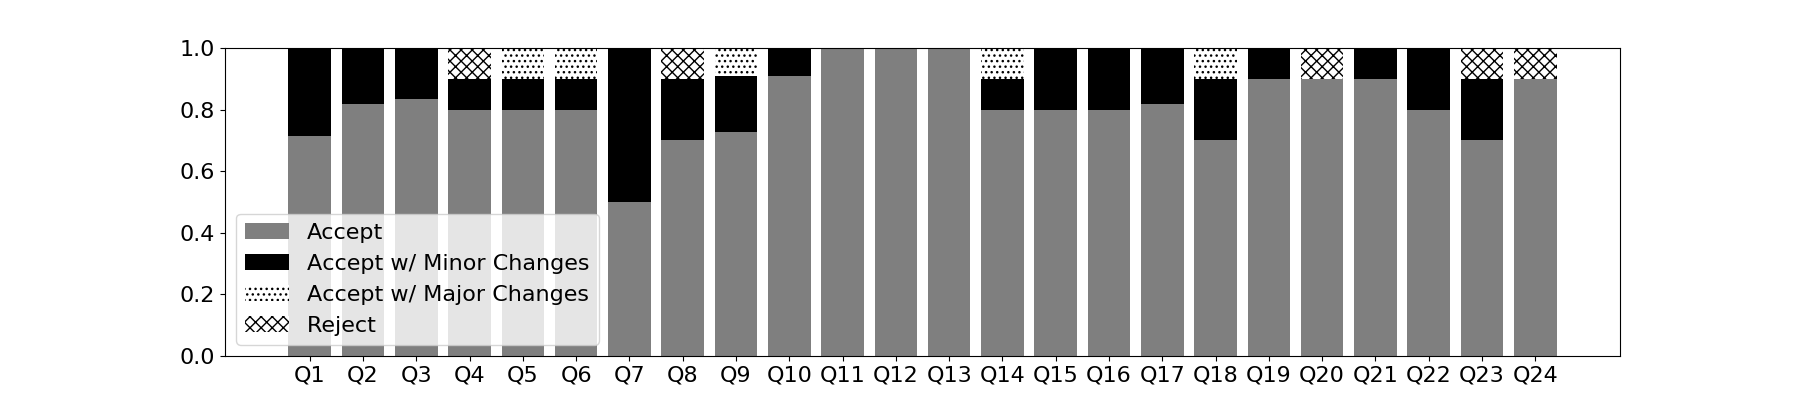
\includegraphics[scale=.4]{images/bar.png}
    \caption{Expert Response to Items}
    \label{fig:accept_rej}
\end{center}
\end{figure}
\fi

\ifshort
\begin{figure}[!htbp]
    \begin{center}
    \advance\leftskip-3cm
    \advance\rightskip-3cm
    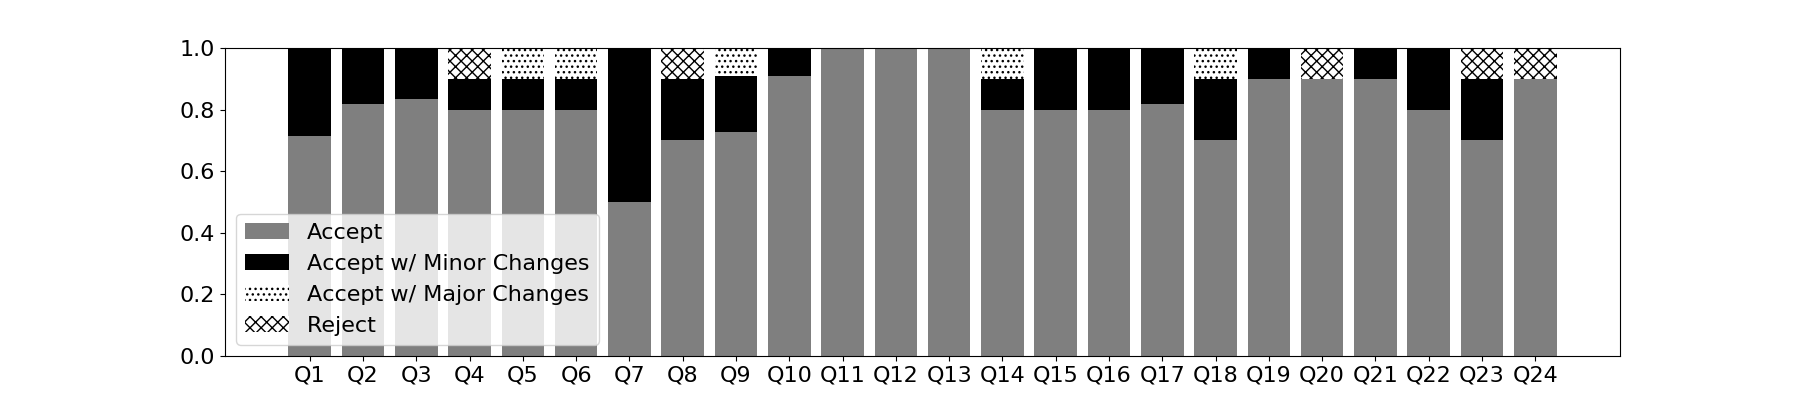
\includegraphics[scale=.3]{images/bar.png}
    \caption{Expert Response to Items}
    \label{fig:accept_rej}
\end{center}
\end{figure}
\fi

\FloatBarrier
\section{Reliability and Standard Error}

Cronbach's $\alpha$ is a measure of the reliability of the instrument. The Cronbach's $\alpha$ of the \gls{cci} in this pilot test is 0.78 which is close to Jorian et al.'s recommendation for good reliability of 0.80 and above Panayiotis's minimum recommendation of 0.70. The reliability of the \gls{cci} is similar to other \glspl{cilabel} as seen in Table \ref{tab:compare}. The reliability of the \gls{cci} suggests that it is sufficiently reliable to be a valid \gls{cilabel}.   


The standard error of measurement defines a confidence interval for each student's true score. The standard measurement error of the \gls{cci} was 2.13 for this pilot test. A 2.13 standard error implies the 68\% confidence interval for a student’s true score, given that a mean observed score of 8.61 points is from 6.48 to 10.74. 

\FloatBarrier

\begin{table*}[!htbp]   
\caption{Comparison with Other Instruments: Concept Assessment Tool for Statics, Statistics Concept Inventory, Dynamics Concept Inventory \cite{jorian}}   
\centering   
\begin{tabular}[width=\textwidth]{ccccc}   
    \toprule
    \textbf{Measurement} & \textbf{\gls{cci}} & \textbf{Statics} & \textbf{Statistics} & \textbf{Dynamics} \\
    \textit{Cronbach's $\alpha$} & 0.78 & 0.84 & 0.64 & 0.74\\   
    \textit{Minimum Difficulty Value} & 0.10 & 0.16 & 0.03 & 0.06 \\   
    \textit{Maximum Difficulty Value} & 0.66 & 0.78 & 0.87 & 0.91 \\   
    \textit{Minimum Discrimination Value} & 0.16 & 0.18 & -0.13 & 0.01\\
    \textit{Maximum Discrimination Value} & 0.47 & 0.65 & -0.57 & 0.56\\   
    \bottomrule   
\end{tabular}   
\label{tab:compare}   
\end{table*}  

\begin{table}[!htbp]
\caption{Instrument Statistics}
\centering
\begin{tabular}{cc}
    \toprule
    \textit{Cronbach's $\alpha$} & 0.78 \\
    \textit{Standard Error of Measurement} & 2.13 \\
    \textit{Mean (Out of 25)} & 8.61\\
    \textit{Standard Deviation} & 4.58\\
    \bottomrule
\end{tabular}
\label{tab:overall}
\end{table}


Cronbach's $\alpha$ can be used as a coarse evaluation of the quality of an item. Each item should increase the quality of the instrument, and excluding that item should decrease the overall reliability. Table \ref{tab:table_cronbach_exclusion} shows the results of the Cronbach calculation with each item excluded. Ideally, every item would be below the original Cronbach $\alpha$ indicating that each item increases the overall reliability. There are no items that decrease the overall reliability and consequently need to be removed.

\iffalse
\iflong
\begin{figure}[ht]
    \begin{center}
    \advance\leftskip-.25cm
    \advance\rightskip-.25cm
    \includegraphics[scale=.5]{images/Cronobach's.png}
    \caption{Cronbach's $\alpha$ with Items Excluded}
    \label{fig:cron}
\end{center}
\end{figure}
\fi
\fi
\input{tex/alpha_table.tex}

\FloatBarrier
\section{Difficulty and Discrimination}

The difficulty of an item is the fraction of students with the correct response. If an item is too hard, the item is separating only strong students from strong students. If an item is too easy, it cannot differentiate any students. The acceptable range of difficulty is between 0.20 and 0.80. The difficulty of each item can be seen in Figure \ref{fig:dif_disc} and Table \ref{tab:diff_v_discrimination}. The range of difficulty for the \gls{cci} is 0.10 to 0.66. When compared to the other instruments the \gls{cci} seen in Table \ref{tab:compare}, it is too difficult and will have less discriminatory power. The \gls{cci} instrument overall is too difficult as evidenced by 21 out of 25 items having difficulty below 0.50 and 5 items falling outside the minimum acceptable difficulty. 

The discrimination of an item indicates the amount of information an item gives about the overall performance of the student. High discrimination indicates that a student's performance on a given item is highly correlated to overall performance. The acceptable range of discrimination is anything above 0.20.  Figure \ref{fig:dif_disc} shows the discrimination of each item. The range of discrimination is 0.16 to 0.47. The discrimination range is not as great as that of other \glspl{cilabel} seen in Table \ref{tab:compare}, but the bottom of the range is much higher than the Statistics Concept Inventory and Dynamics Concept Inventory. The other \glspl{cilabel} had one, ten, and five items fall below the 0.20, while the \gls{cci} had three items below 0.20. The fact that most of the items are above the minimum value is an encouraging indicator that the assessment is valid.   

\iffalse
\iflong
The correlation coefficient can be calculated for each item to quantify how similar the item fits in with the rest of the items. The correlation for each item can be seen in Figure \ref{fig:correlation}. 


\begin{figure}[!hbp]
    \begin{center}
    \advance\leftskip-3cm
    \advance\rightskip-3cm
    \includegraphics[scale=.45]{images/correlation.png}
    \caption{Correlation}
    \label{fig:correlation}
\end{center}
\end{figure}
\fi
\fi

\begin{table}[!htbp]
\caption{Difficulty and Discrimination of Each Item}
\centering
\scalebox{.7}{
\begin{tabular}{cccccc}
    \toprule
    Item & Discrimination & Difficulty & Item & Discrimination & Difficulty\\
    \midrule
    \textit{Q1} & 0.22 & 0.24 & \textit{Q14} & 0.32 & 0.25 \\
    \textit{Q2} & 0.32 & 0.33 & \textit{Q15} & 0.25 & 0.10 \\
    \textit{Q3} & 0.16 & 0.26 & \textit{Q16} & 0.35 & 0.59 \\
    \textit{Q4} & 0.46 & 0.52 & \textit{Q17} & 0.35 & 0.52 \\
    \textit{Q5} & 0.35 & 0.18 & \textit{Q18} & 0.19 & 0.31 \\
    \textit{Q6} & 0.23 & 0.22 & \textit{Q19} & 0.27 & 0.28 \\
    \textit{Q7} & 0.30 & 0.66 & \textit{Q20} & 0.22 & 0.14 \\
    \textit{Q8} & 0.21 & 0.19 & \textit{Q21} & 0.23 & 0.44 \\
    \textit{Q9} & 0.33 & 0.61 & \textit{Q22} & 0.47 & 0.34 \\
    \textit{Q10} & 0.19 & 0.40 & \textit{Q23} & 0.38 & 0.49 \\
    \textit{Q11} & 0.34 & 0.36 & \textit{Q24} & 0.30 & 0.40 \\
    \textit{Q12} & 0.36 & 0.24 & \textit{Q25} & 0.24 & 0.14 \\
    \textit{Q13} & 0.21 & 0.28 & \textit{} &  &\\
    \bottomrule
\end{tabular}
}
\label{tab:diff_v_discrimination}
\end{table}




\begin{figure}[ht]
    \begin{center}
    \advance\leftskip-.25cm
    \advance\rightskip-.25cm
    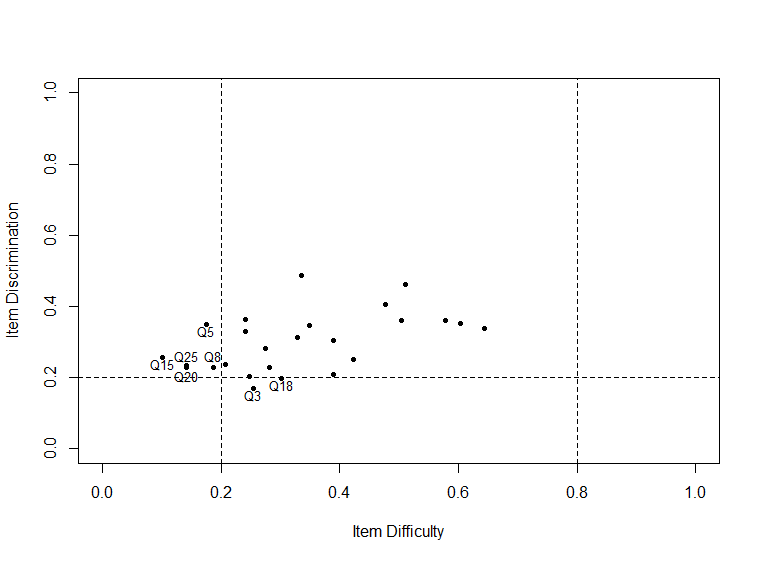
\includegraphics[scale=.45]{images/new_graph.png}
    \caption{Difficulty vs. Discrimination}
    \label{fig:dif_disc}
\end{center}
\end{figure}



\FloatBarrier
\section{Concept Subtests}
The \gls{cci} consists of five concepts: \gls{v}, \gls{c}, \gls{d}, \gls{g}, and \gls{t}. Each item assesses one of these concepts. The individual items within a concept can be grouped and the Cronbach's $\alpha$ calculated to evaluate the reliability of that concept subtest. The $\alpha$'s of the concept subtests are seen in Table \ref{tab:alpha_concept}. When evaluating the concepts, it is notable that all of the values are significantly less than 0.70 which is considered the minimum acceptable value for a reliable instrument \cite{panayiotis}. These findings suggest that the subtests should not be used as evaluations of students' knowledge of the specific concepts. 

%Specifically, \gls{v} has a poor $\alpha$ of 0.236 indicating that the evaluation of that concept through this \gls{cci} is not practical. 

\begin{table}[!htbp]
\caption{Cronbach's $\alpha$ by Concept}
\centering
\scalebox{.8}{
\begin{tabular}{ccc}
    \toprule
    Concept & Cronbach's $\alpha$ & Items Included \\
    \midrule
    \textit{V} & 0.22 & Q1, Q3, Q11, Q17, Q21\\
    \textit{C} & 0.45 & Q2, Q5, Q14, Q18, Q24\\
    \textit{D} & 0.47 & Q4, Q6, Q13, Q19, Q23\\
    \textit{G} & 0.36 & Q8, Q9, Q10, Q22, Q25\\
    \textit{T} & 0.50 & Q7, Q12, Q15, Q16, Q20\\
    \bottomrule
\end{tabular}
}
\label{tab:alpha_concept}
\end{table}


\iflong

The correlation between items in the subtests can be expressed with a correlation matrix. The correlation matrix is the correlation coefficient of each item with every other item. A heat map of the correlation matrix can be seen in Figure \ref{fig:alignment}. The square regions enclose the items in a specific concept subtest. Items within the same concept subtest should be expected to correlate strongly with each other compared to items outside their subtest. We do not see these types of stronger and weaker correlations. 

\begin{figure}[!hbp]
    \centering
    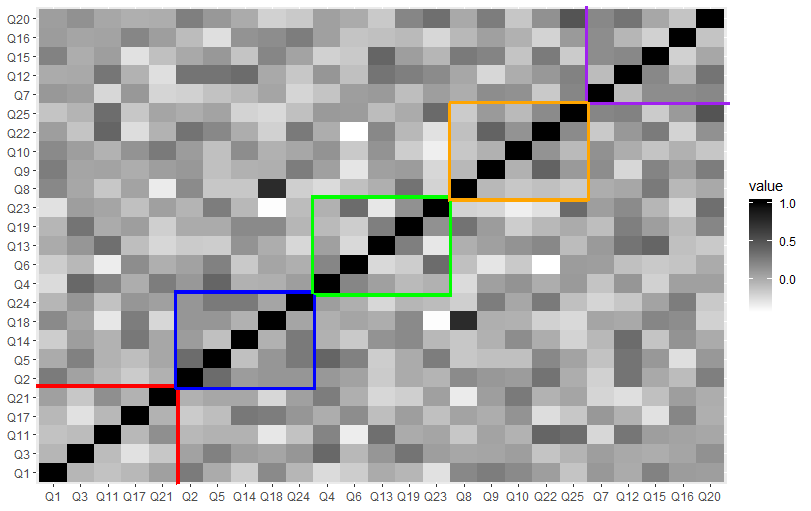
\includegraphics[scale=1.4]{images/heat_map_top_quarter.png}
    \begin{minipage}{0.65\linewidth}
    \tiny
    \emph{
    V: Red,
    C: Blue,
    D: Green,
    G: Orange,
    T: Purple
    }
    \end{minipage}
    \caption{Concept Alignment of Top Quartile}
    \label{fig:alignment}
\end{figure}
\fi

\FloatBarrier
\section{Deeper Analysis of Specific Items}

The psychometric analysis of the \gls{cci} revealed that the instrument has too many difficult items. To inform future revisions of the \gls{cci}, we are analyzing the distractor distribution and distractor discrimination to understand why some items are so difficult. We present an example of this for one of these items, Q15, which had a low difficulty of 0.10 and relatively low discrimination of 0.25 in the pilot trial. We compare Q15 to a stronger item, Q4, which had a good difficulty of 0.52 and discrimination of 0.46 in the pilot trial. 

The distractor analysis shows the proportion of the students' responses in each tertile. The distractor analysis for both Q15 and Q4 can be seen in Table \ref{tab:table_distract}. In Q4, which has a good distribution, the percentage of students getting the correct answer increases from the bottom tertile to the top, and the top tertile generally answers the question correctly. For Q15, although the percentage of students selecting the correct answer increases from the bottom tertile to the top, there is little difference between the top and middle tertiles. Additionally, the top-tertile students answer Q15 correctly 18\% of the time and instead select distractor A 59\% of the time. The preference for option A among the top tertile is causing the item to be too difficult.

\begin{table}[!htbp]
\caption{Distractor Distribution (Asterisk Identifies Correct Alternative)}
\hspace{\fill}
\begin{subtable}[!htbp]{0.45\textwidth}
\flushright
\scalebox{.9}{
\begin{tabular}[!htbp]{c c c c}
\toprule
\textbf{Q4} &  &  &  \\
\midrule
\textit{Response} & \textit{Lower} & \textit{Middle} & \textit{Upper} \\
A & 0.02 & 0 & 0.03 \\
*B & 0.28 & 0.62 & 0.85 \\
C & 0.11 & 0 & 0.26 \\
D & 0.37 & 0.14 & 0 \\
E & .22 & 0.24 & 0.10 \\
blank & 0.02 & 0 & 0 \\
\bottomrule
\end{tabular}
}
\end{subtable}
\hspace{\fill}
\begin{subtable}[!htbp]{0.45\textwidth}
\flushright
\scalebox{.9}{
\begin{tabular}[!htbp]{c c c c}
\toprule
\textbf{Q15} &  &  &  \\
\midrule
\textit{Response} & \textit{Lower} & \textit{Middle} & \textit{Upper} \\
A & 0.22 & 0.36 & 0.59 \\
B & 0.39 & 0.26 & 0.08 \\
C & 0.15 & 0.17 & 0.15 \\
D & 0.22 & 0.05 & 0 \\
*E & 0 & 0.17 & 0.18 \\
blank & 0.02 & 0 & 0 \\
\bottomrule
\end{tabular}
}
\end{subtable}
\label{tab:table_distract}
\end{table}



\iffalse
\hspace{\fill}
\begin{subtable}[!htbp]{0.45\textwidth}
\flushright
\scalebox{.9}{
\begin{tabular}[!htbp]{c c c c}
\toprule
\textbf{Q22} &  &  &  \\
\midrule
\textit{Response} & \textit{Lower} & \textit{Middle} & \textit{Upper} \\
A & 0.06 & 0.02 & 0\\
B & 0.13 & 0.071 & 0.02\\
blank & 0.04 & 0 & 0\\
C & 0.50 & 0.60 & 0.23\\
*D & 0.15 & 0.29 & 0.74\\
E & 0.13 & 0.02 & 0\\
\bottomrule
\end{tabular}
}
\label{tab:table1_d}
\end{subtable}


\begin{subtable}[!htbp]{0.5\textwidth}
\flushright
\scalebox{.9}{
\begin{tabular}[!htbp]{c c c c}
\toprule
\textbf{Q3} &  &  &   \\
\midrule
\textit{Response} & \textit{Lower} & \textit{Middle} & \textit{Upper} \\
A & 0.37 & 0.429 & 0.256 \\
B & 0.13 & 0.238 & 0.128 \\
C & 0.204 & 0.024 & 0.103 \\
*D & 0.204 & 0.214 & 0.436 \\
E & 0.093 & 0.095 & 0.077 \\
blank & 0 & 0 & 0 \\
\bottomrule
\end{tabular}
}
%\caption{\footnotesize Question 3 Distractors}
\label{tab:table1_a}
\end{subtable}
\begin{table}[!htbp]
\caption{Distractor Distribution}
\begin{subtable}[!htbp]{0.5\textwidth}
\flushright
\scalebox{.66}{
\begin{tabular}[!htbp]{c c c c}
\toprule
\textbf{Q3} &  &  &   \\
\midrule
\textit{Response} & \textit{Lower} & \textit{Middle} & \textit{Upper} \\
A & 0.37 & 0.429 & 0.256 \\
B & 0.13 & 0.238 & 0.128 \\
C & 0.204 & 0.024 & 0.103 \\
*D & 0.204 & 0.214 & 0.436 \\
E & 0.093 & 0.095 & 0.077 \\
blank & 0 & 0 & 0 \\
\bottomrule
\end{tabular}
}
%\caption{\footnotesize Question 3 Distractors}
\label{tab:table1_a}
\end{subtable}
\hspace{\fill}
\begin{subtable}[!htbp]{0.5\textwidth}
\flushright
\scalebox{.66}{
\begin{tabular}[!htbp]{c c c c}
\toprule
\textbf{Q5} &  &  &   \\
\midrule
\textit{Response} & \textit{Lower} & \textit{Middle} & \textit{Upper} \\
A & 0.389 & 0.524 & 0.308 \\
B & 0.167 & 0.071 & 0.051 \\
C & 0.278 & 0.167 & 0.128 \\
D & 0.074 & 0.167 & 0.077 \\
*E & 0.093 & 0.071 & 0.436 \\
blank & 0 & 0 & 0 \\
\bottomrule
\end{tabular}
}
\label{tab:table1_b}
\end{subtable}
\hspace{\fill}
\begin{subtable}[!htbp]{0.5\textwidth}
\flushright
\scalebox{.66}{
\begin{tabular}[!htbp]{c c c c}
\toprule
\textbf{Q8} &  &  &  \\
\midrule
\textit{Response} & \textit{Lower} & \textit{Middle} & \textit{Upper} \\
A & 0.333 & 0.357 & 0.154 \\
B & 0.463 & 0.31 & 0.513 \\
*C & 0.074 & 0.238 & 0.333 \\
D & 0.074 & 0 & 0 \\
E & 0.056 & 0.095 & 0 \\
blank & 0 & 0 & 0 \\
\bottomrule
\end{tabular}
}
\label{tab:table1_c}
\end{subtable}
\hspace{\fill}
\begin{subtable}[!htbp]{0.5\textwidth}
\flushright
\scalebox{.66}{
\begin{tabular}[!htbp]{c c c c}
\toprule
\textbf{Q15} &  &  &  \\
\midrule
\textit{Response} & \textit{Lower} & \textit{Middle} & \textit{Upper} \\
A & 0.222 & 0.357 & 0.59 \\
B & 0.389 & 0.262 & 0.077 \\
C & 0.148 & 0.167 & 0.154 \\
D & 0.222 & 0.048 & 0 \\
*E & 0 & 0.167 & 0.179 \\
blank & 0.019 & 0 & 0 \\
\bottomrule
\end{tabular}
}
\label{tab:table1_d}
\end{subtable}
\hspace{\fill}
\begin{subtable}[!htbp]{0.5\textwidth}
\flushright
\scalebox{.66}{
\begin{tabular}[!htbp]{c c c c}
\toprule
\textbf{Q20} &  &  &  \\
\midrule
\textit{Response} & \textit{Lower} & \textit{Middle} & \textit{Upper} \\
A & 0.222 & 0.143 & 0 \\
*B & 0.074 & 0.167 & 0.231 \\
C & 0.333 & 0.262 & 0.308 \\
D & 0.222 & 0.119 & 0.051 \\
E & 0.093 & 0.31 & 0.41 \\
blank & 0.056 & 0 & 0 \\
\bottomrule
\end{tabular}
}
\label{tab:table1_e}
\end{subtable}
\hspace{\fill}
\begin{subtable}[!htbp]{0.5\textwidth}
\flushright
\scalebox{.66}{
\begin{tabular}[!htbp]{c c c c}
\toprule
\textbf{Q25} &  &  &  \\
\midrule
\textit{Response} & \textit{Lower} & \textit{Middle} & \textit{Upper} \\
*A & 0.093 & 0.095 & 0.282 \\
B & 0.241 & 0.286 & 0.205 \\
C & 0.259 & 0.19 & 0.128 \\
D & 0.167 & 0.167 & 0.128 \\
E & 0.204 & 0.262 & 0.256 \\
blank & 0.037 & 0 & 0 \\
\bottomrule
\end{tabular}
}
\label{tab:table1_f}
\end{subtable}
\label{tab:table_distract}
\end{table}
\fi

 
 Table \ref{tab:table_distract_discrim} shows the distractor discrimination value for both Q4 and Q15. We expect the distractors to have negative discrimination values. Q4 has negative or zero distractor discrimination values for each distractor as well as a large positive discrimination value for the correct answer. Q15 does have a large positive discrimination for the correct answer and is even above the minimum acceptable value, but distractor A has a larger, positive discrimination value. This analysis reveals that for some reason the correct answer is not compelling to the strongest students, suggesting that the wording or structure of the answer choices may be to blame. We explore this assertion more in future work.

\begin{table}[!ht]
\caption{Distractor Discrimination Values (Asterisk Identifies Correct Alternative)}
\hspace{\fill}
\begin{subtable}[!htbp]{0.45\textwidth}
\flushright
\scalebox{1}{
\begin{tabular}[!htbp]{c c}
\toprule
\textbf{Q4} &  \\
\midrule
\textit{Distractor} & \textit{Discrimination} \\
A & 0 \\
*B & 0.46 \\
C & -0.14 \\
D & -0.26 \\
E & -0.04 \\
\bottomrule
\end{tabular}
}
\label{tab:table4_c}
\end{subtable}
\hspace{\fill}
\begin{subtable}[!htbp]{0.45\textwidth}
\flushright
\scalebox{1}{
\begin{tabular}[!htbp]{c c}
\toprule
\textbf{Q15} & \\
\midrule
\textit{Distractor} & \textit{Discrimination} \\
A & 0.35  \\
B & -0.19 \\
C & 0 \\
D & -0.26 \\
*E & 0.24  \\
\bottomrule
\end{tabular}
}
\label{tab:table4_d}
\end{subtable}
\label{tab:table_distract_discrim}
\end{table}



\iffalse

\hspace{\fill}
\begin{subtable}[!htbp]{0.45\textwidth}
\flushright
\scalebox{1}{
\begin{tabular}[!htbp]{c c}
\toprule
\textbf{Q22} & \\
\midrule
\textit{Distractor} & \textit{Discrimination} \\
A & -0.09 \\
B & -0.09 \\
C & -.08 \\
*D & 0.47 \\
E & -0.14 \\
\bottomrule
\end{tabular}
}
\label{tab:table4_d}
\end{subtable}
\begin{subtable}[!htbp]{0.5\textwidth}
\flushright
\scalebox{1}{
\begin{tabular}[!htbp]{c c}
\toprule
\textbf{Q3} &   \\
\midrule
\textit{Distractor} & \textit{Discrimination} \\
A & -0.0465  \\
B & 0.0618 \\
C & -0.152 \\
*D & 0.169\\
E & -0.028 \\
\bottomrule
\end{tabular}
}
%\caption{\footnotesize Question 3 Distractors}
\label{tab:table4_b}
\end{subtable}

\fi

%\glsresetall
\chapter{Discussion}
This validation study revealed the instrument could be used to evaluate cybersecurity but would benefit from minor modifications. The \gls{cci} has many good properties: high reliability and strong expert consensus on the suitability of all items. Unfortunately, our findings revealed a few weaknesses of the \gls{cci} as currently constructed: low reliability for individual concepts, items that are too difficult, and too many difficult items on the instrument.

From the results of the pilot trial, the \gls{cci} had very high reliability, especially when compared to other \glspl{cilabel}. The Cronbach's $\alpha$ is 0.78, which is considered good for a \gls{cilabel}. In addition to the \gls{cci} reliability, no items decrease the overall $\alpha$. Not reducing the $\alpha$ indicates the individual items are all measuring the same construct of cybersecurity conceptual knowledge \cite{dlci}. The reliability of the instrument is necessary for the instrument to be valid but not sufficient.

Experts positively reviewed each item and provided feedback to improve the items. Experts also provided suggestions for improving the wording and distractors of each item. We used this feedback to select the 25 items that had the strongest consensus of quality from the experts. The expert reviews provide evidence for the content validity of the \gls{cci} by demonstrating that multiple cybersecurity instructors believe that the \gls{cci} items represent conceptual knowledge that students should have after a first course in cybersecurity. 

\glsreset{c}

The strengths of the \gls{cci} indicate that the collection of items and individual items are well designed from an instructor perspective and reliable from a student performance perspective. However, the student response data reveals that there is still room for improvement. Notably, while we designed the \gls{cci} to assess five concepts, the student performance data did not align well with these five concepts. For example, there is no consistent correlation of the items within each concept subtest. Additionally, the items that constitute a subtest have low reliability; each $\alpha$ for the individual concept subtest is below 0.50 \cite{jorian}. Because of the low reliability of the concept subtests, we cannot recommend using the concept subtests to assess students' knowledge of each concept individually.

There are two possible interpretations for this lack of correlation and reliability within the concept subtests. First, it is possible that the items were poorly designed and do not reflect the core concepts. Second, it is possible that the concepts themselves are poorly bounded, interconnected, or too complex. Given that the expert reviewers did not express any concerns about the content of the items, we argue that the second interpretation is more likely. 

Our finding of low cohesion among concept subtests is a common finding among previously published \glspl{cilabel} \cite{jorian}. The commonality of this finding suggests that it is generally difficult for designers of an instrument to design effective concept subtests. While most items may primarily engage students in one concept, the concepts are likely interconnected. Students need to use multiple concepts to answer each item correctly. We believe that this fact may be especially true in cybersecurity, which requires individuals to consider the motivations or capabilities of attackers, constraints or goals of defenders, and the technologies or techniques needed to mitigate risk.

Additionally, the concepts discovered in the Delphi process may be too complex and are really culminations of similar, but separate, concepts \cite{delphi}. For example, concept \gls{c} involves four unique forms of attack. A confidentiality attack could cover attacking a secure message protocol. An availability attack could cover a denial of service attack. Both of these examples are forms of attack and both of them are very relevant to cybersecurity. A student, however, may understand mechanisms that enable secure communications and still have very little idea about denial-of-service attacks. Thus each item of the \gls{cci} must be multifaceted and creating subtests will be difficult, if not intractable, without creating isomorphic, redundant questions.


%In future iterations, it may be useful to split these concepts up into smaller concepts or use heuristics. \gls{efa} can find underlying relations between exam constructs. These heuristics will be useful with more students to explore potential concept groupings.

If we want to create reliable and valid concept subtests, we may need to consider other models for creating them. For example, we could try narrowing the scope of concept \gls{c} to just one attribute (e.g., confidentiality). This option may not be desirable because it ignores the complexity of an attacker's varied motivations. Alternatively, we could create multiple instruments that more fully explore each of the five core concepts, but this option would dramatically increase the work and cost of creating instruments for cybersecurity. As currently constructed, the \gls{cci} provides a reliable instrument for measuring a students' overall understanding of cybersecurity, which is a much-needed first step. Future work can explore which types of future development are needed for creating these subtests.

Unlike the alignment of the concepts, a good range of difficulty is often achieved in published \glspl{cilabel} and necessary for the instrument to be valid. The \gls{cci} is skewed to be too difficult: five items are more difficult than the recommended level of difficulty, and for 21 out of 25 items, fewer than 50\% of students answered each item correctly. This degree of difficulty suggests that some items need to be made easier to improve our ability to distinguish between students with varying abilities and knowledge. Future work on the \gls{cci} must explore how to effectively make some items easier to improve the quality of the \gls{cci}.  

\section{Limitations}

There are a number of limitations in the pilot trial. The most notable limitation is the depth of analysis performed on the pilot trial results. \gls{irt} is not practical with the number of students in the trial but would enable deeper analysis. Additionally, because the Cronbach's $\alpha$ for each concept subtest was so low, we did not perform measurements such as \gls{cfa} and \gls{efa}.  These limitations are acceptable because this study is a pilot test.


There were also limitations in the number of students from each university. Ideally, there would be a similar number of representatives from the different types of universities so that the results were not skewed toward University A. The localization may have biased the findings to one university.

\section{Future Work}

We will take Q15 as a specific example of the type of modification we will make to the difficult items. Less than 10\% of students answered Q15 correctly, far below what is acceptable for a \gls{cilabel}. \glsreset{v}

The item covers finding vulnerabilities in a defense and falls under concept \gls{v}. The scenario describes a hypothetical nuclear treaty between two countries that requires a method of securely transmitting a message from a monitoring device. Neither country trusts the other, and the design must be fair to each country. There are certain properties the solution must hold. Both parties want assurances that the message is not modified. Country A wants to ensure that the message originates from the device. Country B wants to monitor the message data in real time. The premise is: ``The sender applies a keyed cryptographic hash function to each message using a key distributed only to the sender, Country A, and Country B." Students are expected to find potential vulnerabilities in the suggested outputs of the device.

Option A is the message with a hash of the message and the current time. Options B, C, and D are the key and a hash of the message, the message, and hash of the message, and the hash of the message respectively. Option E, the correct answer, is that the design cannot satisfy the system requirements. 

Our distractor analysis revealed that the best students chose Option A more than the correct answer. This finding reveals that, as students' knowledge increased, this wrong answer became more compelling. When constructed well, each item should lead students to pick the correct answer more often as their knowledge increases.

The preference for Option A is understandable given that it is more reasonable than the other 3 options. Options B and D do not even send the original message so the message cannot be verified. Option A and Option C do not guarantee that the source is sending the message and since each party has the key they can modify the message and attach a new hash. Because A has the same structure as C with the addition of time being sent, it appears to be strictly superior to C making it the best option. Students must see the problems with each option and select Option E which serves as a ``none of the above." Including a ``none of the above" in general makes assessments harder \cite{none_of_above}, especially with Option A and C satisfying some of the desired properties. 

The problem with the item, and further ``none of the above" in general, is that Option E makes no assertion. This fact leads students to pick the most reasonable of the other choices. We have modified this item, changing Option E to make an assertion. The new Option E is ``The design does not work because Countries A and B can modify the message." This allows students a definitive assertion to test and come to the same conclusion that the other options do not satisfy the requirements. We anticipate that this change, while being minor, will make the item easier and differentiate more students.

After making similar modifications to other items, our next work is to administer the instrument to more students and reanalyze the results. With the easier items, the difficulty will cover a better range and better separate students. The range of difficulties and modification of items that are too difficult should increase the discriminatory power of the \gls{cci} and improve the \gls{cci}'s validity and usefulness.


%\glsresetall
\chapter{Conclusion}
%The pilot trial for the \gls{cci} included 142 students from 6 universities. The \gls{cci} had very good reliability and support from the expert panel. There suggested modifications include changing items to make them easier and to re-evaluate the individual concepts after scaling up to more students. The next step is to make the proper modifications and then administering the \gls{cci} to more students in a full trial. 

The purpose of the expert review and pilot trial was to evaluate the validity of the \gls{cci}. The expert review and pilot testing of the \gls{cci} revealed the \gls{cci} reliably tests students' knowledge of cybersecurity. At this point, the \gls{cci} could be used as an evaluation instrument but the scores would be low, reducing the discriminatory power of the assessment. By making the \gls{cci} easier, we will be able to create an assessment that should be broadly applicable and provide useful measurements of a broad range of cybersecurity students. Further research will cover the modifications of the items and testing with more students. 



%%%%%%%%%%%%%%%%%%%%%%%%%%%%%%%%%%%%%%%%%%%%%%%%%%%%%%%%%%%%%%%%%%%%%%%%%%%%%%%
% APPENDIX
%


\backmatter

\addtocontents{toc}{\protect\setcounter{tocdepth}{1}}

%%%%%%%%%%%%%%%%%%%%%%%%%%%%%%%%%%%%%%%%%%%%%%%%%%%%%%%%%%%%%%%%%%%%%%%%%%%%%%%
% BIBLIOGRAPHY
%
% Put references in BibTeX format in thesisrefs.bib.
\bibliographystyle{IEEE_ECE}
% Put references in BibTeX format in thesisrefs.bib.
\bibliography{thesisrefs}

\clearpage
\setcounter{table}{0}
\renewcommand{\thetable}{A.\arabic{table}}
\appendix
\chapter{Appendix A Item Details}
\input{tex/apx1}
\chapter{Appendix B Full Assessment}
\FloatBarrier
\begin{figure}[!ht]
    \begin{center}
    \advance\leftskip-3cm
    \advance\rightskip-3cm
    \includegraphics[scale=.25]{images/exam/correctly_formated_exam-01.jpg}
    \label{fig:correctly_formated_exam-01}
\end{center}
\end{figure}

\begin{figure}[!ht]
    \begin{center}
    \advance\leftskip-3cm
    \advance\rightskip-3cm
    \includegraphics[scale=.25]{images/exam/correctly_formated_exam-02.jpg}
    \label{fig:correctly_formated_exam-02}
\end{center}
\end{figure}

\begin{figure}[!ht]
    \begin{center}
    \advance\leftskip-3cm
    \advance\rightskip-3cm
    \includegraphics[scale=.25]{images/exam/correctly_formated_exam-03.jpg}
    \label{fig:correctly_formated_exam-03}
\end{center}
\end{figure}
\begin{figure}[!ht]
    \begin{center}
    \advance\leftskip-3cm
    \advance\rightskip-3cm
    \includegraphics[scale=.25]{images/exam/correctly_formated_exam-04.jpg}
    \label{fig:correctly_formated_exam-04}
\end{center}
\end{figure}
\begin{figure}[!ht]
    \begin{center}
    \advance\leftskip-3cm
    \advance\rightskip-3cm
    \includegraphics[scale=.25]{images/exam/correctly_formated_exam-05.jpg}
    \label{fig:correctly_formated_exam-05}
\end{center}
\end{figure}
\begin{figure}[!ht]
    \begin{center}
    \advance\leftskip-3cm
    \advance\rightskip-3cm
    \includegraphics[scale=.25]{images/exam/correctly_formated_exam-06.jpg}
    \label{fig:correctly_formated_exam-06}
\end{center}
\end{figure}

\begin{figure}[!ht]
    \begin{center}
    \advance\leftskip-3cm
    \advance\rightskip-3cm
    \includegraphics[scale=.25]{images/exam/correctly_formated_exam-07.jpg}
    \label{fig:correctly_formated_exam-07}
\end{center}
\end{figure}

\begin{figure}[!ht]
    \begin{center}
    \advance\leftskip-3cm
    \advance\rightskip-3cm
    \includegraphics[scale=.25]{images/exam/correctly_formated_exam-08.jpg}
    \label{fig:correctly_formated_exam-08}
\end{center}
\end{figure}

\begin{figure}[!ht]
    \begin{center}
    \advance\leftskip-3cm
    \advance\rightskip-3cm
    \includegraphics[scale=.25]{images/exam/correctly_formated_exam-09.jpg}
    \label{fig:correctly_formated_exam-09}
\end{center}
\end{figure}

\begin{figure}[!ht]
    \begin{center}
    \advance\leftskip-3cm
    \advance\rightskip-3cm
    \includegraphics[scale=.25]{images/exam/correctly_formated_exam-10.jpg}
    \label{fig:correctly_formated_exam-10}
\end{center}
\end{figure}

\begin{figure}[!ht]
    \begin{center}
    \advance\leftskip-3cm
    \advance\rightskip-3cm
    \includegraphics[scale=.25]{images/exam/correctly_formated_exam-11.jpg}
    \label{fig:correctly_formated_exam-11}
\end{center}
\end{figure}

%%%%%%%%%%%%%%%%%%%%%%%%%%%%%%%%%%%%%%%%%%%%%%%%%%%%%%%%%%%%%%%%%%%%%%%%%%%%%%%
% AUTHOR'S BIOGRAPHY
% As of 10/03/2011, Author's Biography or Vita no longer accepted by Grad College

\end{document}
\endinput
